%!TEX root = ./main.tex
%
% This file is part of the i10 thesis template developed and used by the
% Media Computing Group at RWTH Aachen University.
% The current version of this template can be obtained at
% <http://www.media.informatik.rwth-aachen.de/karrer.html>.

\chapter{Introduction}
Cancer is one of the leading causes of death around the globe. It is considered to be the most complex disease that human species has to deal with. It is characterized by undesirable growth in cells which are caused by changes in genomes and exposure to environment\cite{5}. Each cancer type has unique architecture of genetic variation - somatic mutations, copy number alterations, gene expression profiles and different epigenetic aberration. Therefore, a strong need for better diagnosis, personalized medicines for patients have arose, which correlates with better understanding of changes at genetic level in tumors. All thanks to technological advancements in high-throughput techniques for genome-wide interrogations such as Microarray and Next-Generation Sequecing(NGS) platforms have provided wealth of multi-disciplinary, multi-institutional pilot projects in cancer studies\cite{stratton2009cancer} \cite{lengauer1998genetic}.\\~\\
Various unique projects catering to cancer genome study such as 1000 Genome Project\cite{10002010map}\cite{10002012integrated}, Encyclopedia of DNA Elements Project (ENCODE)\cite{ecker2012genomics}, Immunological Genome Project (ImmGen)\cite{shay2013immunological}, The Cancer Genome Atlas (TCGA)\cite{lee2016exploring} which aims at investigating biological systems at several levels and creating humongous datasets with different data types. These projects motivates the bioinformaticians to develop novel data integration methodologies in order to explore hidden insights. With respect to current state-of-the-art for data integration platforms, data lake promises to addresses the onslaught of Big Data generated across the projects. However, one of the biggest challenges in data lake is to prevent turning into a data swamp or silos. Moreover, especially for cancer genomic data, where the users must have a first hand knowledge in biomedical area since its metadata alone cannot provide the full meaning of respective data. There are dearth of novel methodologies that can point out,for example - genes with name "TP53" and "BCC7" or "Breast Cancer" and "Breast Tumor" means the same. Additionally, in context of conceptual hierarchy, the patient's clinical data set has a broader term as a Person or narrower terms such as Outgoing, Incoming or Doner.  Thus, the use of knowledge organization system from both biomedical domain as well as generic is needed in order to understand the data much more unambiguously.  This would assist the users to find, explore, understand, and trust the data better. Such domain knowledge and thesauri are captured as specification of conceptualization(or commonly known as ontologies) in BioPortal\cite{noy2009bioportal}, Simple Knowledge Organization Systems(SKOS)\cite{miles2005skos}. \\~\\
The current data lake efforts that are on data quality have the following features - profiling, cleaning and data enrichment. Keeping in consideration of our work in relation to semantic recognition of descriptive data schema, we focus on profiling aspect. But, existing profiling capabilities revolves around statistical data profiling and do not offer semantic aspect. This motivates us to an idea of enabling semantic profiling in data lakes. \\~\\
Semantic Profiling is a methodology that exploits semantic-based tools and ontologies in order to derive lucid understanding of the information being stored in current systems. This approach is much more rigorous than former traditional profiling techniques for the following reasons: \\
i) Unlike traditional profiling which captures as much anomalies as you can until you stop, whereas, in semantic profiling once you select the domain of study, you stick by the rules and guidelines. \\
ii) If a user perform semantic profiling on one system and would like to combine the results of first system  with those from other system, it can easily be facilitated through its feature of reusability. \\
iii) Semantic profiling allows setting up of testing hypothesis to monitor the data lake in production scenario which can detect semantic drift.\\~\\
Therefore, through this thesis work, we extend current profiling efforts in the data lake solutions in a much more rigorous way i.e. through semantical enrichment using ontologies[\ref{fig:Figure1}]. This would open the door in answering questions about data sources like: 
\begin{itemize}
	\item Does the data adhere to particular standards such as gene and disease ontologies?
	\item  Is there a way to capture controlled vocabularies, taxonomies and thesauri for clinical dataset of patients?
\end{itemize}
\begin{figure}[htbp]
	% center the image.
	\centering
	
	% include a png file. Adapt size to 0.5 * textwidth and retain aspect ratio (!)
	%	\resizebox{\textwidth}{!}{Figure1.png}}
	% NOTE: if possible do not include bitmap graphics in your paper, if available use
	% a vector graphics format
	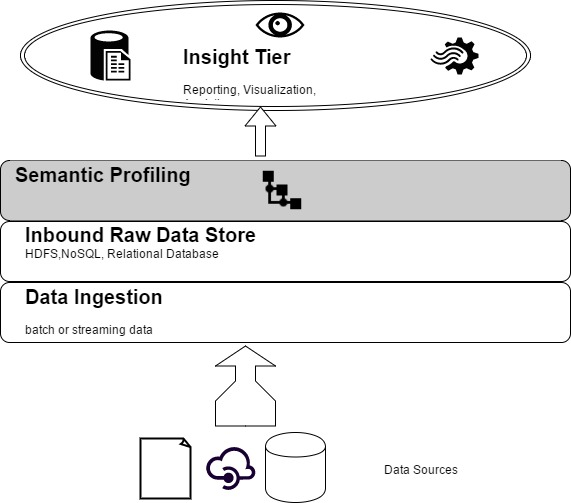
\includegraphics[scale=0.6]{./images/datalake.JPG}
	\caption{Need to extend the current semnantic tendencies of data lake}
	\label{fig:Figure1}
\end{figure}

\section{Thesis Goals \& Outcome}
\label{goals}
Specific aims of my thesis are as follows:
\begin{itemize}
	\item Extend current profiling efforts in our state-of-art data lake, which only offers statistical analysis, to semantic indicators that provides the following features:
	\subitem{a)} capture reports of all the bugs - different existing anomalies in the data source
	\subitem{b)} set of update actions applied to the data source - translation to the same concept or format
	\subitem{c)} semantic data structure with meta-information - in form  of ontologies (for example, BioPortal, SKOS), data dictionary, regular expressions and flags to determine the type of profiling
	\item  Develop a fully customizable dashboard with:
	 \subitem{a)} provenance adhering to IT standards
	   \subitem{b)} governance at entity level 

\end{itemize}